\documentclass[tikz,border=2pt]{standalone}
\usepackage{amsmath}
\usepackage{pgfplots}
\pgfplotsset{compat=1.18}
\usetikzlibrary{calc}

\begin{document}
% Increasing: x<y gives f(x)<=f(y); the flat piece is allowed (non-decreasing) but not for a
% strictly increasing function. The right panel is decreasing.
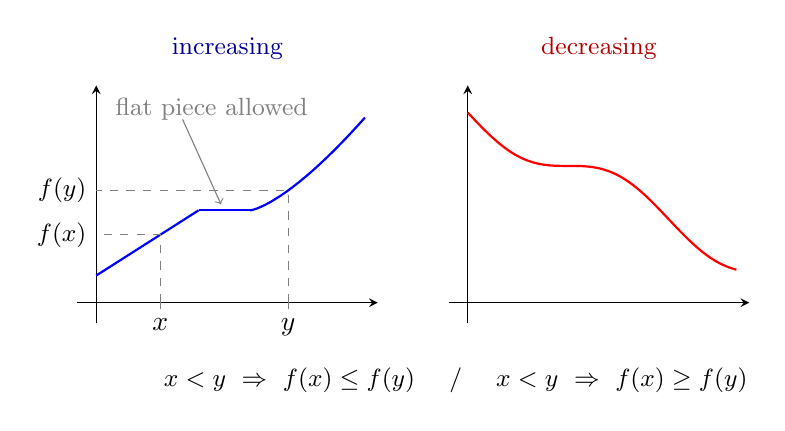
\begin{tikzpicture}
	\begin{axis}[
		name=left,
		axis lines=middle,
		xmin=-0.3, xmax=4.4,
		ymin=-0.3, ymax=3.2,
		xtick={1,3}, xticklabels={$x$,$y$},
		ytick=\empty,
		xlabel={}, ylabel={},
		samples=120, smooth, clip=false,
		width=5.4cm, height=4.6cm,
		title={increasing}, title style={blue!60!black, font=\small}
		]
		\addplot[thick, blue, domain=0:1.6] {0.4+0.6*x};
		\addplot[thick, blue, domain=1.6:2.4] {1.36};
		\addplot[thick, blue, domain=2.4:4.2] {1.36+0.6*(x-2.4)^1.4};
		\draw[dashed, gray] (axis cs:1,0) -- (axis cs:1,1.0) -- (axis cs:0,1.0);
		\draw[dashed, gray] (axis cs:3,0) -- (axis cs:3,{1.36+0.6*0.6^1.4}) -- (axis cs:0,{1.36+0.6*0.6^1.4});
		\node[anchor=east, font=\small] at (axis cs:0,1.0) {$f(x)$};
		\node[anchor=east, font=\small] at (axis cs:0,{1.36+0.6*0.6^1.4}) {$f(y)$};
		\node[gray, anchor=north west, font=\small] at (axis cs:0.15,3.15) {flat piece allowed};
		\draw[gray, ->] (axis cs:1.35,2.7) -- (axis cs:1.95,1.45);
	\end{axis}
	\begin{axis}[
		at={(left.east)}, anchor=west, xshift=0.9cm,
		axis lines=middle,
		xmin=-0.3, xmax=4.4,
		ymin=-0.3, ymax=3.2,
		xtick=\empty, ytick=\empty,
		samples=120, smooth, clip=false,
		width=5.4cm, height=4.6cm,
		title={decreasing}, title style={red!70!black, font=\small}
		]
		\addplot[thick, red, domain=0:4.2] {2.8-0.5*x-0.25*sin(deg(2*x))};
	\end{axis}
	\node[font=\small, anchor=north] at ($(left.south)+(2.9,-0.45)$) {$x<y\ \Rightarrow\ f(x)\le f(y)$ \quad / \quad $x<y\ \Rightarrow\ f(x)\ge f(y)$};
\end{tikzpicture}
\end{document}
